\begin{figure}[h]
  % parametri
  \def \r{1.5}
  \def \h{2}
  \def \e{0.4}
  \def \d {1}
  % sotto-figura 1
  \begin{subfigure}{0.48\textwidth}
    \centering
    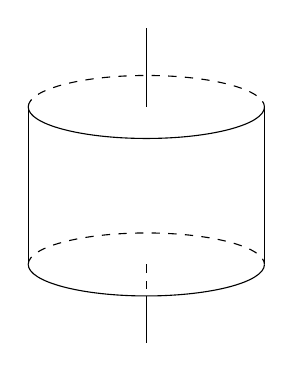
\begin{tikzpicture}
      % ellissi
      % Armatura superiore
      \draw (-\r,\h) arc[start angle=180, end angle=360, x radius=\r, y radius=\e];
      \draw[dashed] (-\r,\h) arc[start angle=180, end angle=0, x radius=\r, y radius=\e];

      % Armatura inferiore
      \draw (-\r,0) arc[start angle=180, end angle=360, x radius=\r, y radius=\e];
      \draw[dashed] (-\r,0) arc[start angle=180, end angle=0, x radius=\r, y radius=\e];
      
      % Fili verticali
      \draw (0,\h) -- (0,\h+1);
      \draw [dashed] (0,0) -- (0,-\e);
      \draw (0,-\e) -- (0,-1);

      % bordi cavità
      \draw (\r, 0) -- (\r , \h);
      \draw (-\r, 0) -- (-\r , \h);
    \end{tikzpicture}
    \caption{Cavità cilindrica}
    \label{figure:_cavità:_A}

  \end{subfigure} % lasciare una riga vuota fa andare a capo la seconda figura (e \hfill)
  \hfill
  % sotto-figura 2
  \begin{subfigure}{0.48\textwidth}
    \centering
    \begin{tikzpicture}

      \def \hb {1.5*\h}
      \def \l {0.3}
      \begin{scope}[shift = {(0,1)}]
        \draw (0,0) -- (0,\hb) -- (\d,\hb) -- (\d,0) -- (0,0);
        % circuito amperiano tratteggiato con frecce
        \draw [dashed, decorate, decoration={mark=at position 0.5 with {\arrow[triangle 45]{>}}}] (-\l, \hb/4) -- (-\l,\hb* 3/4);
        \draw [dashed, decorate, decoration={mark=at position 0.5 with {\arrow[triangle 45]{>}}}] (-\l,\hb* 3/4) -- (\l, \hb * 3/4);
        \draw [dashed, decorate, decoration={mark=at position 0.5 with {\arrow[triangle 45]{>}}}] (\l, \hb * 3/4) -- (\l, \hb/4 );
        \draw [dashed, decorate, decoration={mark=at position 0.5 with {\arrow[triangle 45]{>}}}] (\l, \hb/4 ) -- (-\l , \hb/4);
      \end{scope}
      % Aggiungo una linea invisibile per "riempire" lo spazio sotto
      \path[draw=none] (0,0) -- (0,2);
      % Etichette
      \node at (-\l - 0.3 ,\hb/4 + 1.2) {$\gamma$};
      \node at (\d/2,0.7) {$\delta$};
    \end{tikzpicture}
    \caption{Sezione della cavità e circuito amperiano}
    \label{figure:_cavità:_B}
  \end{subfigure}
\end{figure}
